\documentclass{article}

\usepackage{graphicx}

\begin{document}
\newpage
   \vspace*{\stretch{1.0}}
   \begin{center}
      \Large\textbf{Earth 436B Thesis}\\
      \large\textit{John Lawson}
   \end{center}
   \vspace*{\stretch{2.0}}

\newpage

\section{Locations}   
-Grand Traverse Bay, Michigan (GTB)\\
-Au Train Bay, Michigan (ATB)\\
-Batchawana Bay, Ontario (BATB)\\
-Tahquamenon Bay, Michigan (TAHB)\\
\newpage
\section{Method}
-OSL dating used to determine age for sequences of late Holocene shoreline
deposits, (known as Strandplain sequences) at each site vs current day elevation.\\
-Not all strandplains were age dated due to cost, so a linear regression model of age vs horizontal distance along the strandplain sequence is used to estimate age values for strandplains that were not directly age dated.\\
-This is then used to create a graph of elevation vs time for each site\\
\newpage
\section[2]{Method}
-OSL dating used to determine age for sequences of Quaternary beach deposits (strandplain sequences) at each site vs current day elevation.\\
-This is then used to create a graph of elevation vs time for each site\\
\begin{figure}[h]
	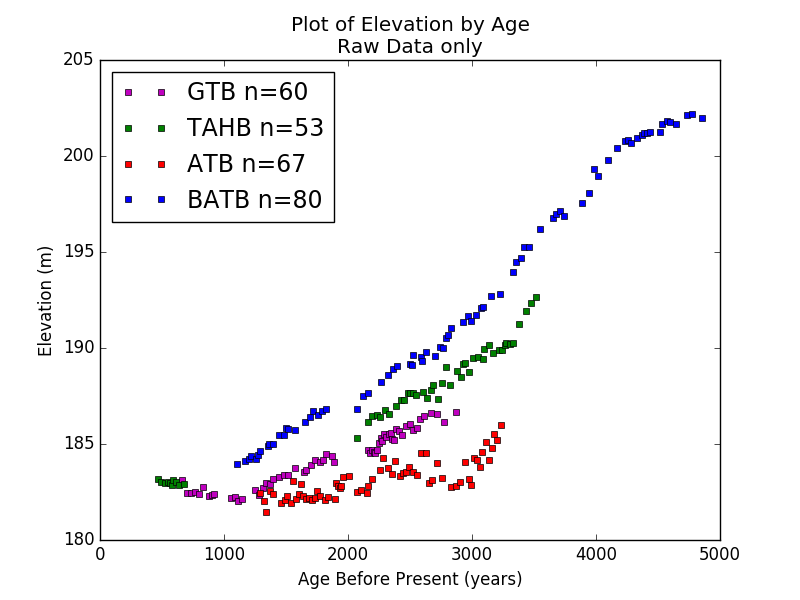
\includegraphics[width=1.1\linewidth]{data/theDataRaw.png}
	\caption{Current day elevation of relict shorelines with respect to time before present over the last 5000 years. Strandplain sites Au Train Bay, Michigan (ATB), Batchawana Bay, Ontario (BATB), Tahquamenon Bay, Michigan (TAHB), and Grand Traverse Bay, Michigan (GTB) surrounding Lake Superior are plotted individually. Data from Johnston et al, (2012)}
	\label{fig:rawData}
\end{figure} 
%\begin{figure}[h]
	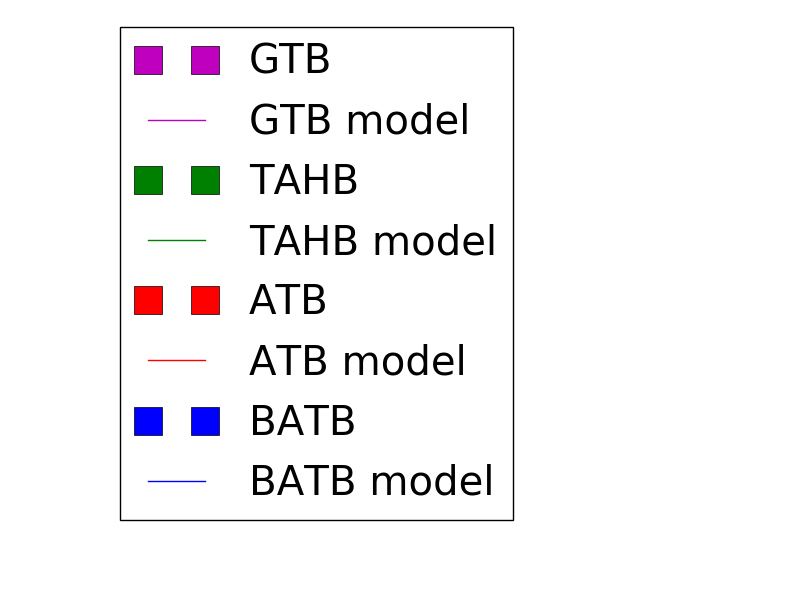
\includegraphics[width=0.40\textwidth]{data/legendary.png}
	%\makebox[\textwidth]{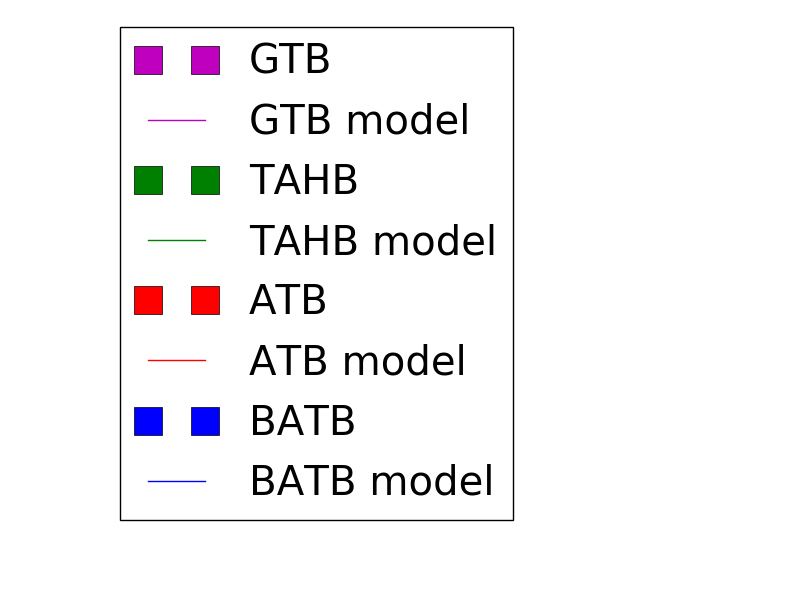
\includegraphics[width=\paperwidth]{data/legendary.png}}
	%\caption{Site Legend}
	%\label{fig:rdmLegend}
\end{figure}


\newpage
\section[2]{Method}
-Data not available continuously for each site, or at the same time for each site to compare gia, so values must be inferred using linear interpolation between known data points.\\
\begin{figure}[h]
	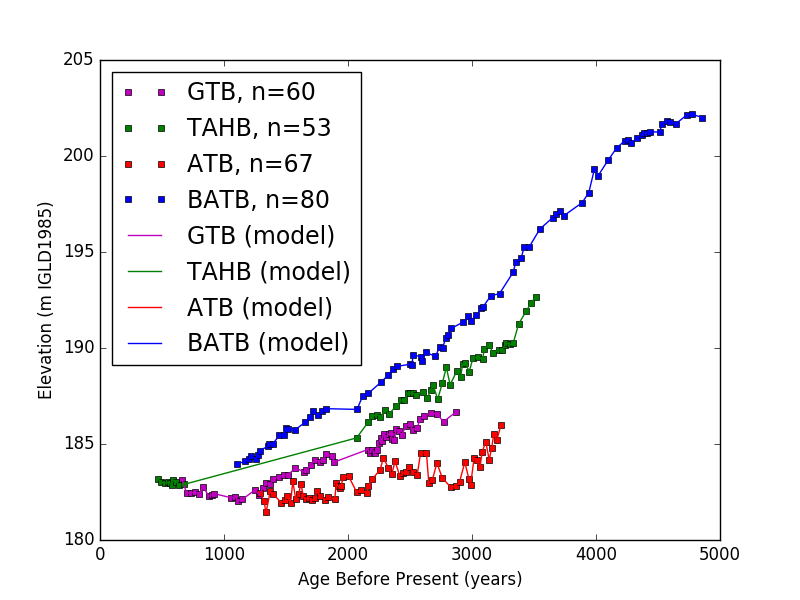
\includegraphics[width=\linewidth]{data/theData.png}
	\caption{Water surface elevation with respect to time before present, modelled}
	\label{fig:rawDataWithModel}
\end{figure}
\newpage
%\begin{figure}[h]
	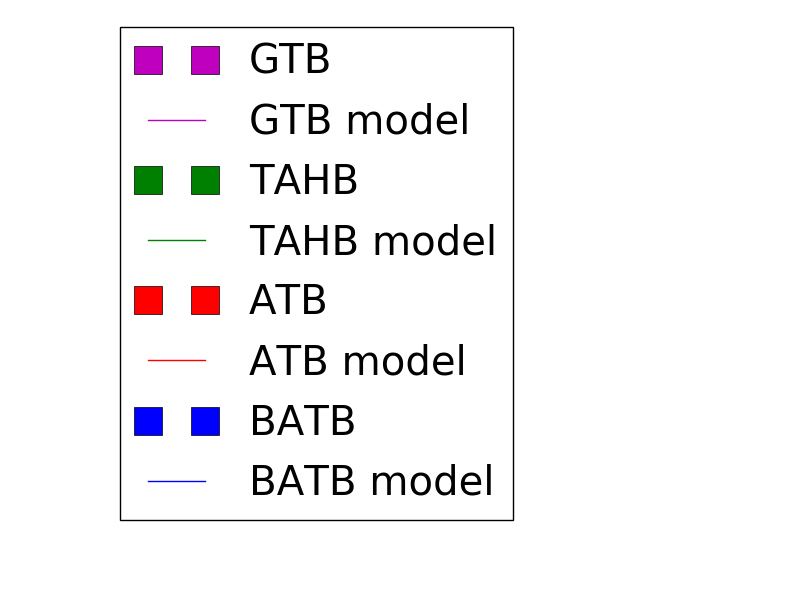
\includegraphics[width=0.40\textwidth]{data/legendary.png}
	%\makebox[\textwidth]{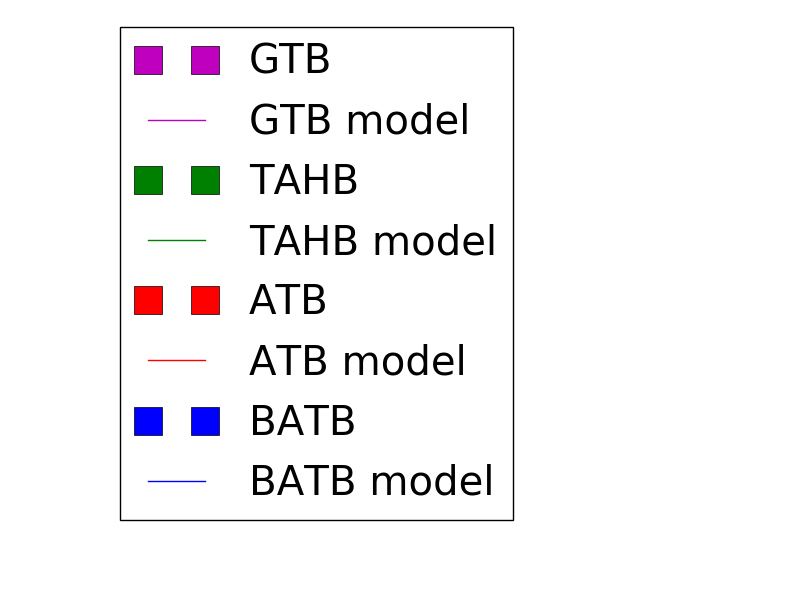
\includegraphics[width=\paperwidth]{data/legendary.png}}
	%\caption{Site Legend}
	%\label{fig:rdmLegend}
\end{figure}


\newpage
\section[2]{Method}
-GIA is now plotted by subtracting between the measured values of one dataset and the modelled value of another.\\
-6 combinations of pairs of sites are created, each of which has a forward (A to B) and backward (B to A) comparison.\\


\newpage
\begin{figure}[t]
	\makebox[\textwidth]{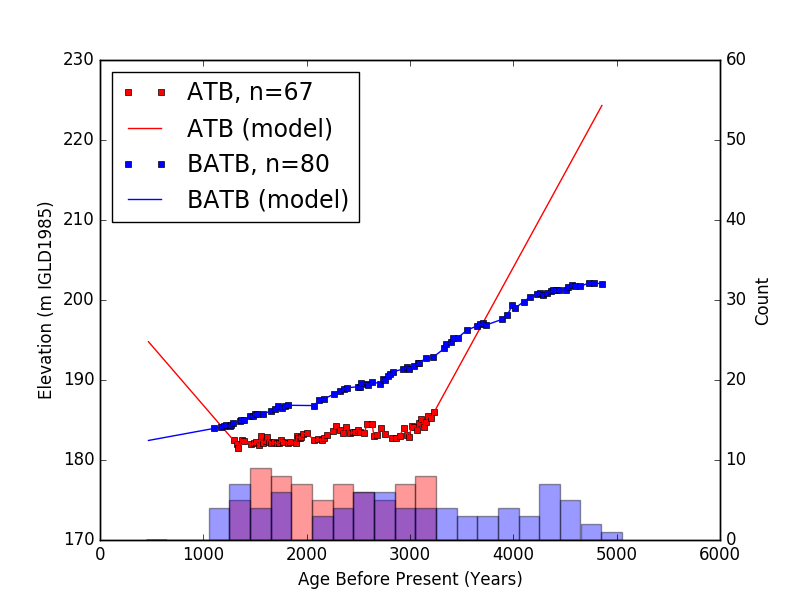
\includegraphics[width=0.72\paperwidth]{data/ATB-BATB_DataAndModel.png}}
	\caption{ATB-BATB raw data with linear interpolation model}
	\label{fig:data_ATBxBATB}
\end{figure}
\newpage

\begin{figure}[t]
	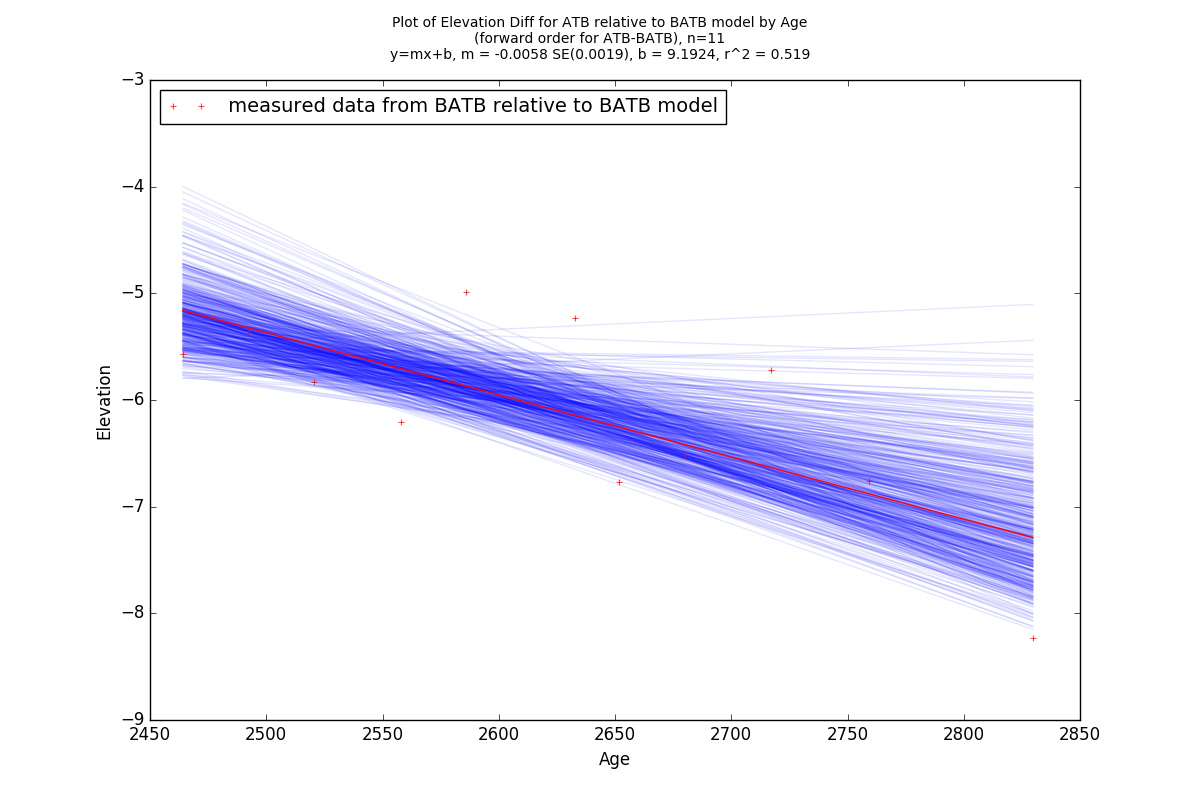
\includegraphics[width=0.9\linewidth]{data/gias/theGIA_ATB_relative_to_BATB.png}
	\caption{Differences in elevation measured from the ATB data to the ATB model}
	\label{fig:gias_ATBxBATB}
\end{figure}
\newpage


\begin{figure}[t]
	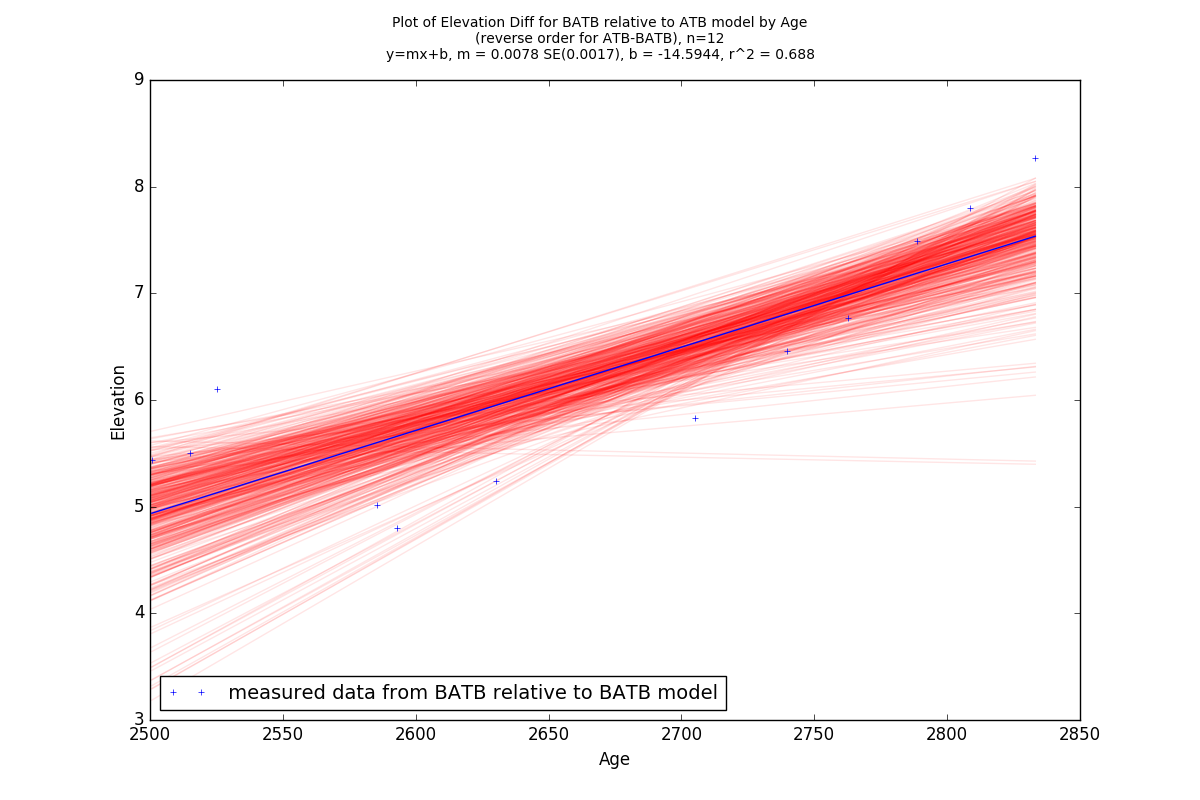
\includegraphics[width=0.9\linewidth]{data/gias/theGIA_BATB_relative_to_ATB.png}
	\caption{Differences in elevation measured from the BATB data to the ATB model}
	\label{fig:gias_BATBxATB}
\end{figure}
\newpage
% this desperately needs to be done as a loop



\begin{figure}[h]
	\makebox[\textwidth]{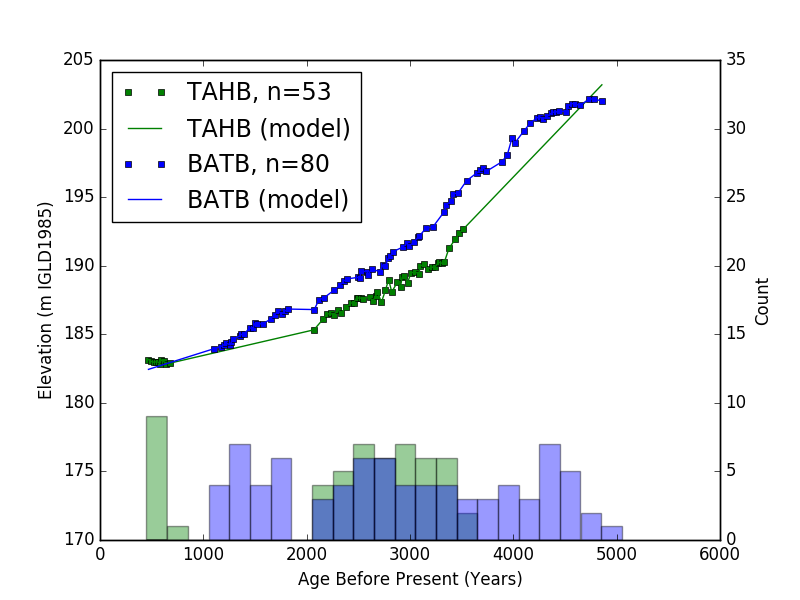
\includegraphics[width=0.72\paperwidth]{data/TAHB-BATB_DataAndModel.png}}
	\caption{TAHB-BATB raw data with linear interpolation model}
	\label{fig:data_TAHBxBATB}
\end{figure}
\newpage

\begin{figure}[h]
	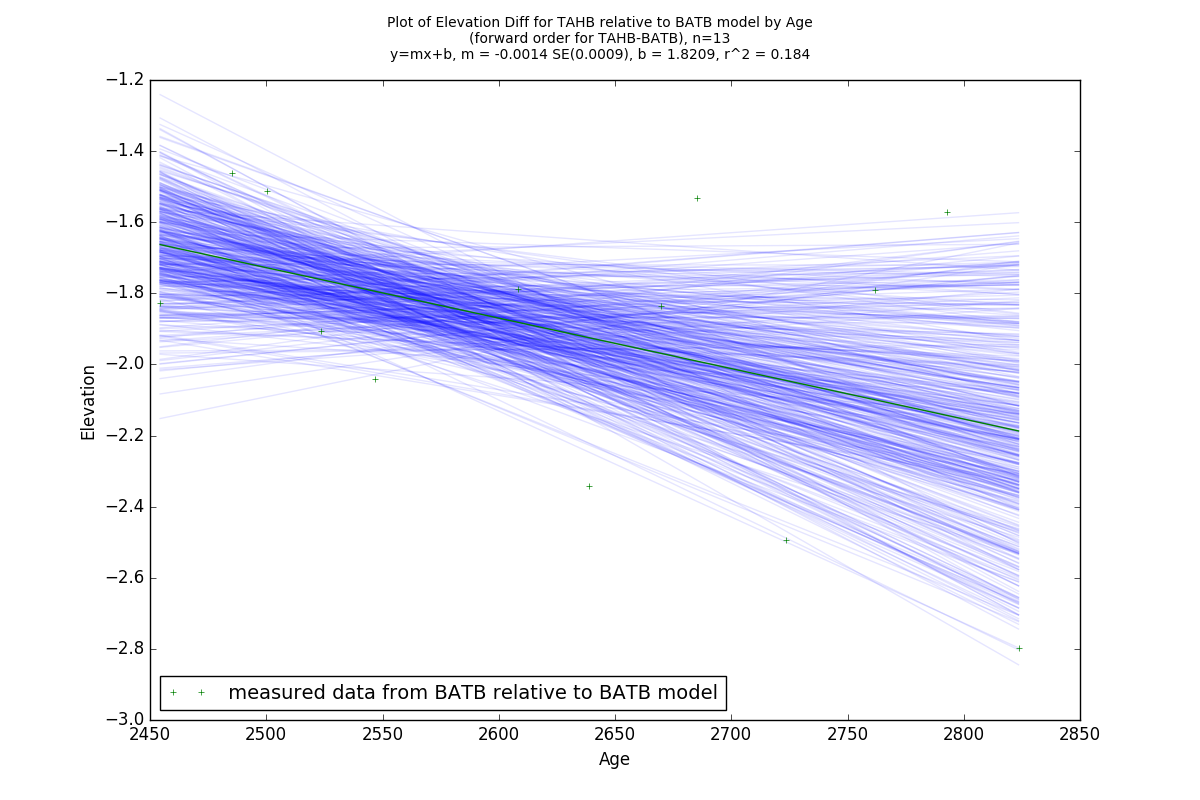
\includegraphics[width=0.9\linewidth]{data/gias/theGIA_TAHB_relative_to_BATB.png}
	\caption{Differences in elevation measured from the TAHB data to the BATB model}
	\label{fig:gias_TAHBxBATB}
\end{figure}
\newpage


\begin{figure}[h]
	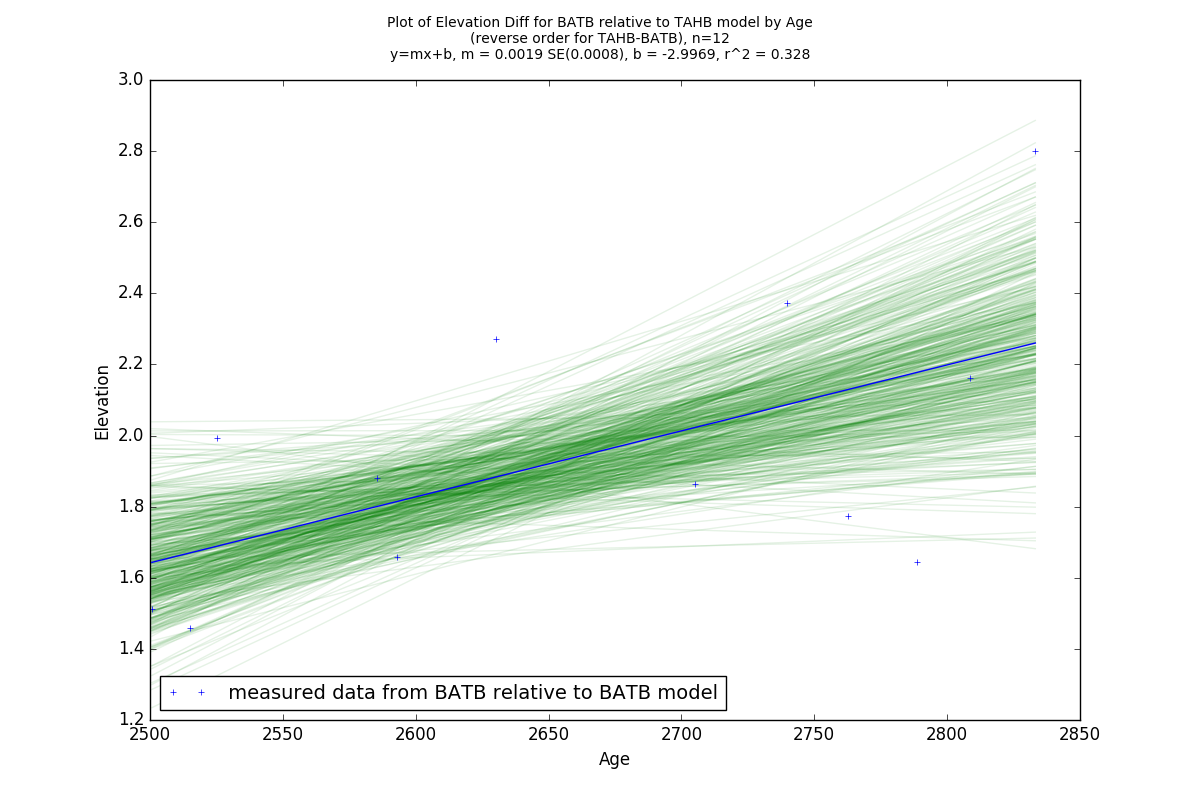
\includegraphics[width=0.9\linewidth]{data/gias/theGIA_BATB_relative_to_TAHB.png}
	\caption{Differences in elevation measured from the BATB data to the TAHB model}
	\label{fig:gias_BATBxTAHB}
\end{figure}
\newpage








\begin{figure}[h]
	\makebox[\textwidth]{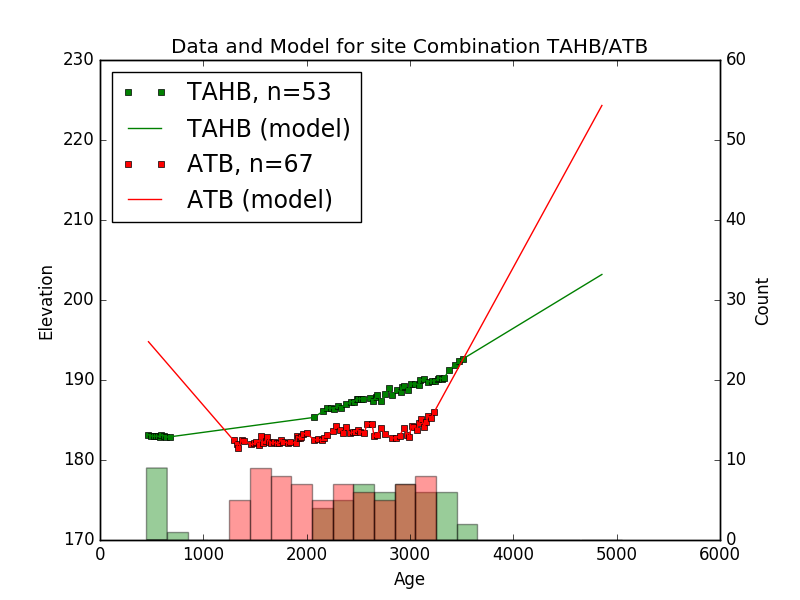
\includegraphics[width=0.72\paperwidth]{data/TAHB-ATB_DataAndModel.png}}
	\caption{TAHB-ATB raw data with linear interpolation model}
	\label{fig:data_TAHBxATB}
\end{figure}
\newpage

\begin{figure}[h]
	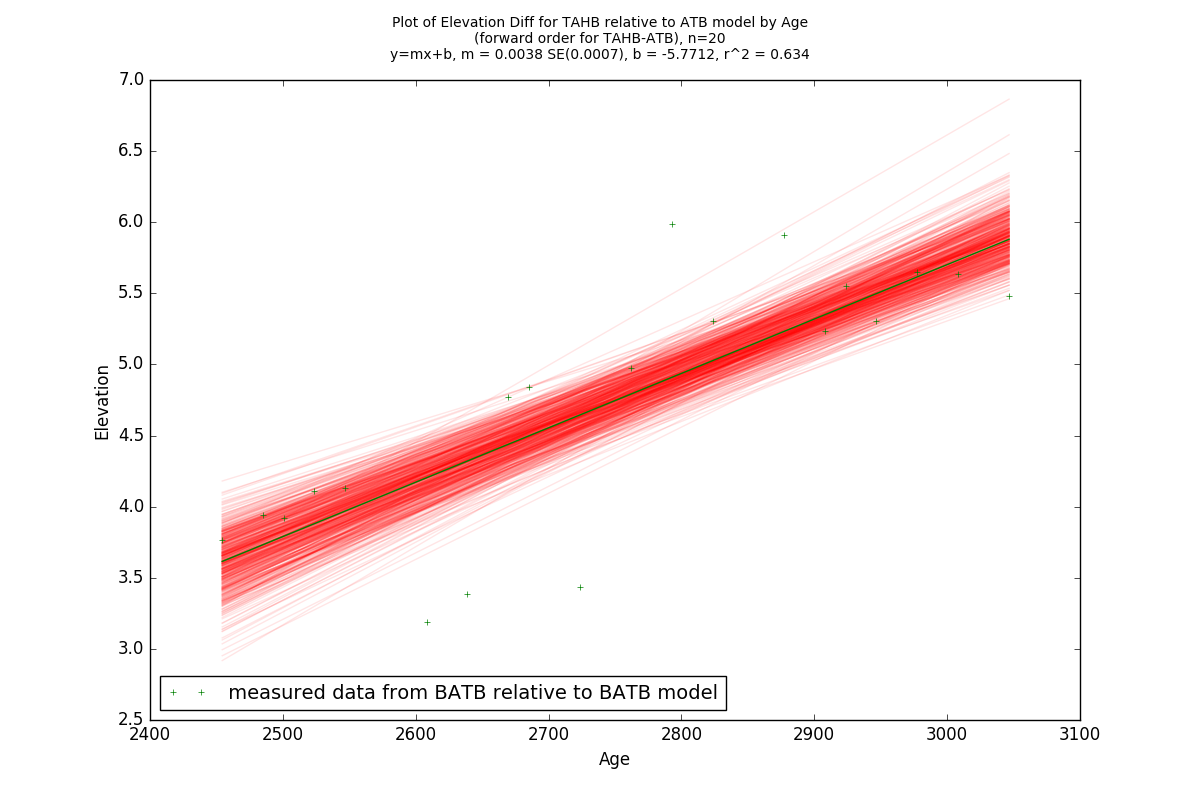
\includegraphics[width=0.9\linewidth]{data/gias/theGIA_TAHB_relative_to_ATB.png}
	\caption{Differences in elevation measured from the TAHB data to the ATB model}
	\label{fig:gias_TAHBxATB}
\end{figure}
\newpage


\begin{figure}[h]
	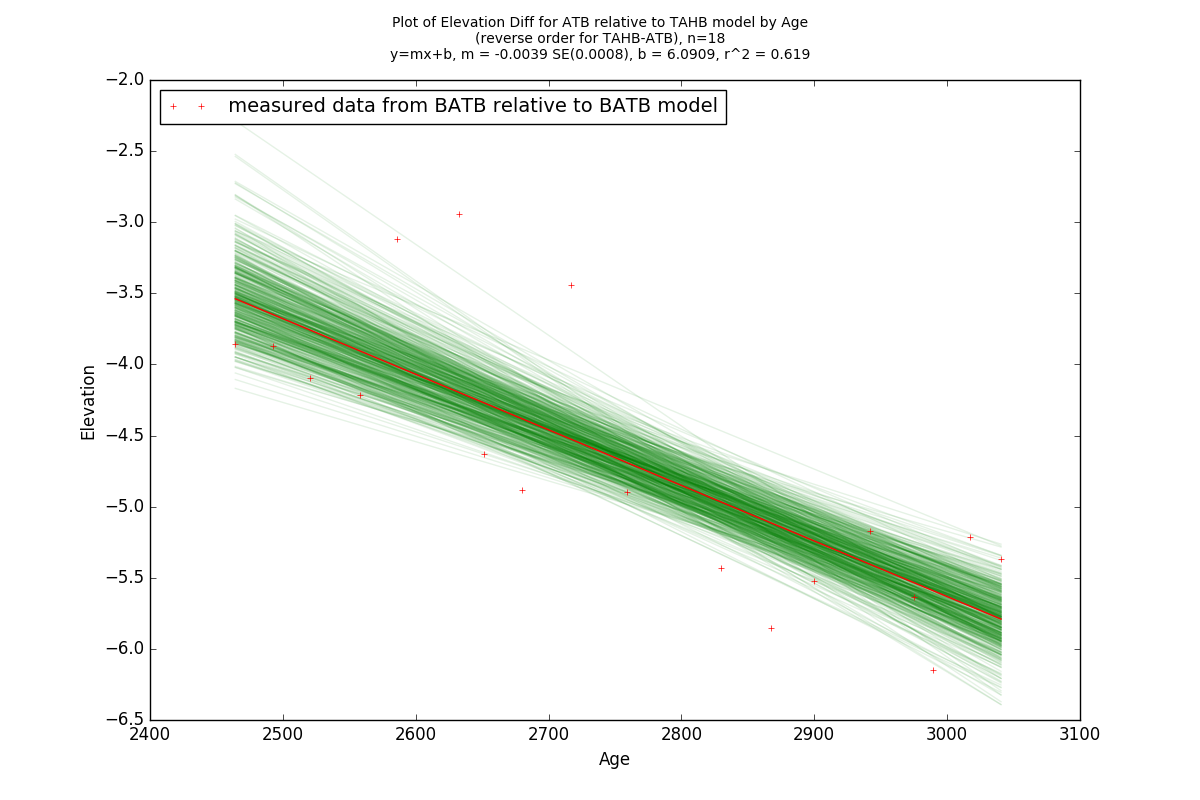
\includegraphics[width=0.9\linewidth]{data/gias/theGIA_ATB_relative_to_TAHB.png}
	\caption{Differences in elevation measured from the ATB data to the TAHB model}
	\label{fig:gias_ATBxTAHB}
\end{figure}
\newpage






\begin{figure}[h]
	\makebox[\textwidth]{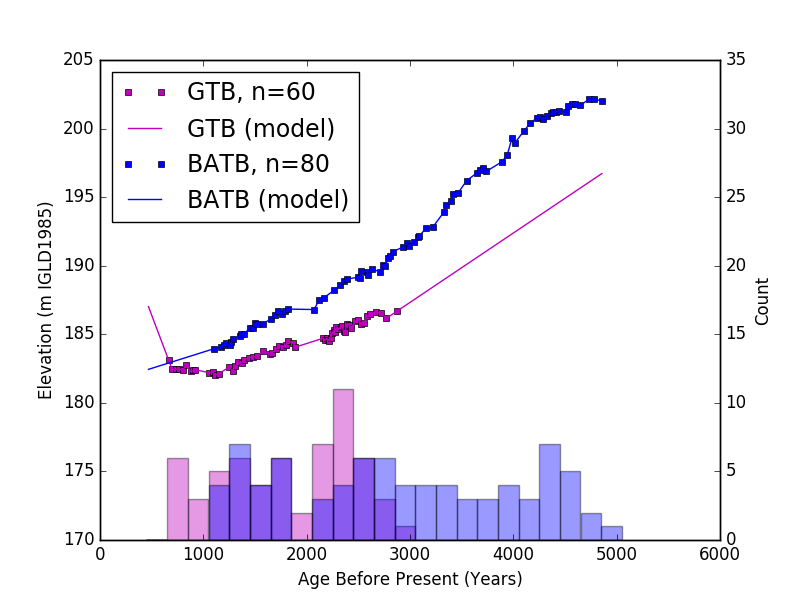
\includegraphics[width=0.72\paperwidth]{data/GTB-BATB_DataAndModel.png}}
	\caption{GTB-BATB raw data with linear interpolation model}
	\label{fig:data_GTBxBATB}
\end{figure}
\newpage

\begin{figure}[h]
	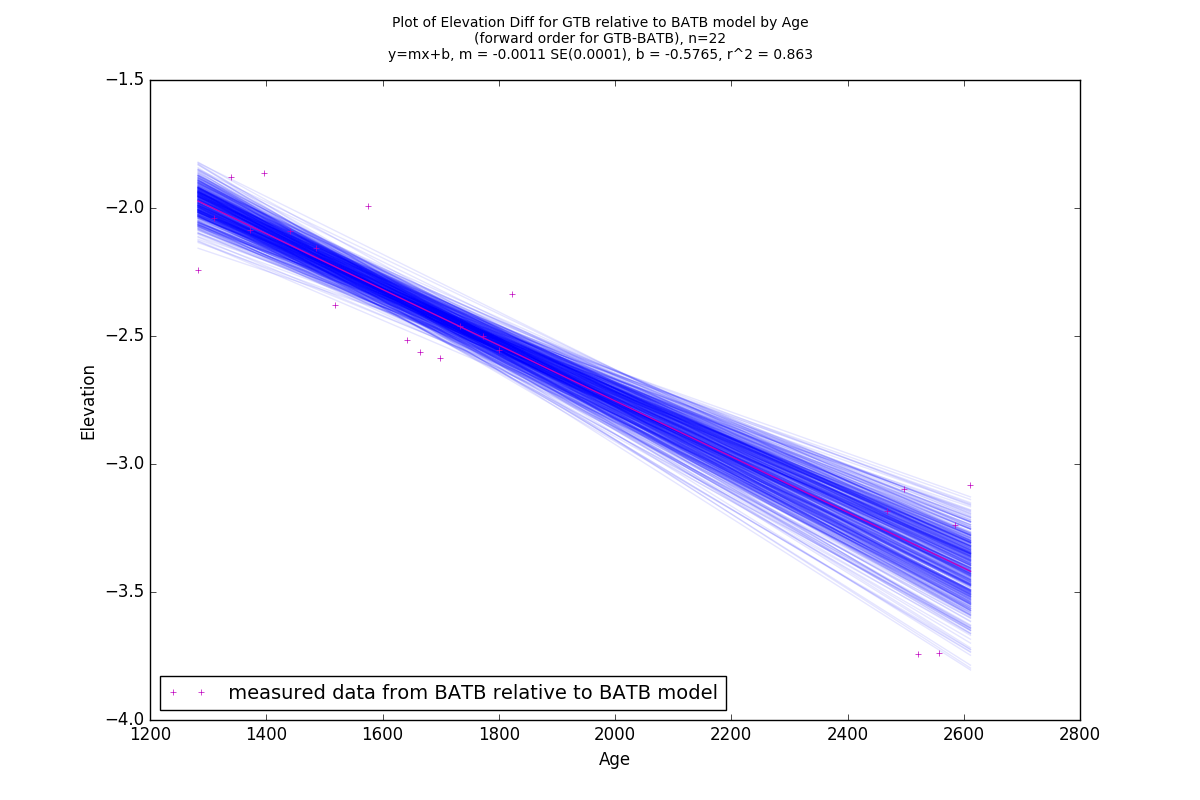
\includegraphics[width=0.9\linewidth]{data/gias/theGIA_GTB_relative_to_BATB.png}
	\caption{Differences in elevation measured from the GTB data to the BATB model}
	\label{fig:gias_GTBxBATB}
\end{figure}
\newpage


\begin{figure}[h]
	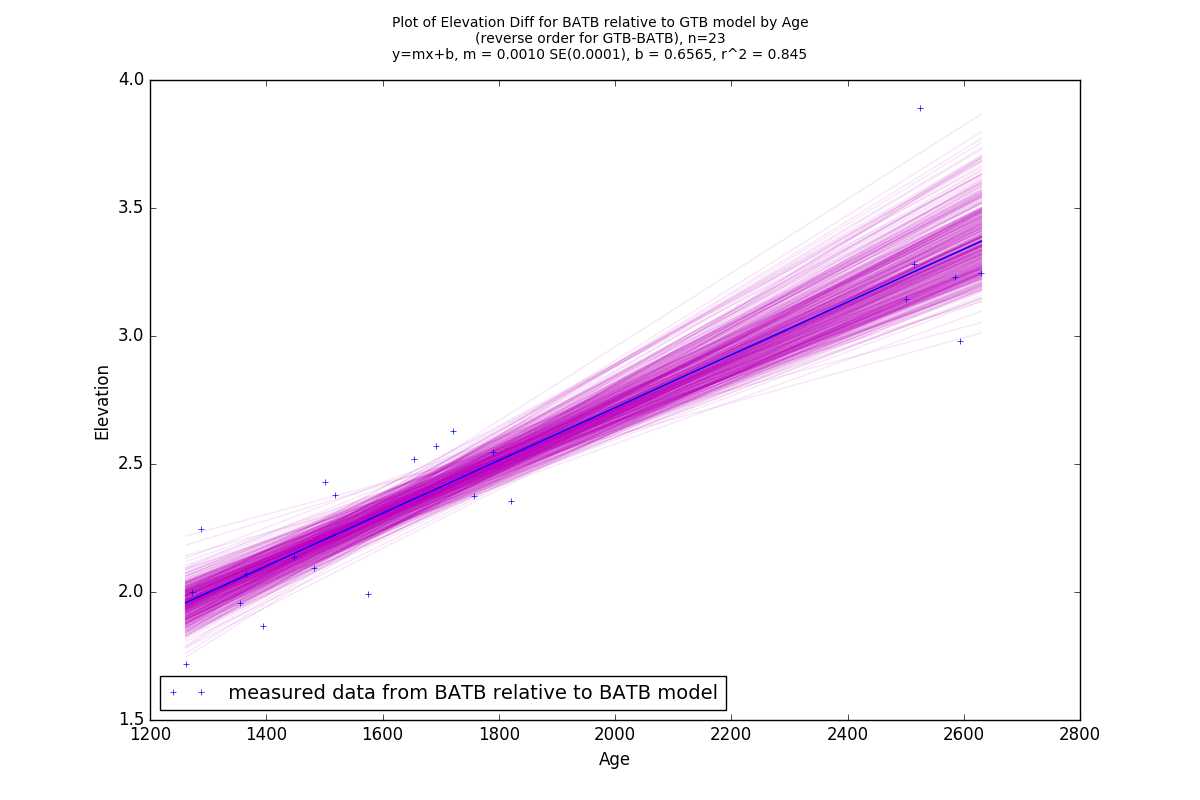
\includegraphics[width=0.9\linewidth]{data/gias/theGIA_BATB_relative_to_GTB.png}
	\caption{Differences in elevation measured from the BATB data to the GTB model}
	\label{fig:gias_BATBxGTB}
\end{figure}
\newpage









\begin{figure}[h]
	\makebox[\textwidth]{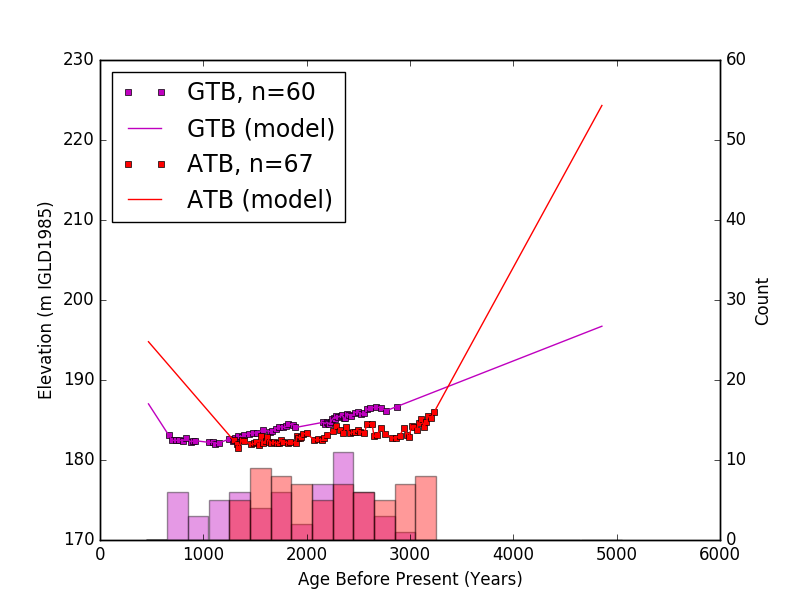
\includegraphics[width=0.72\paperwidth]{data/GTB-ATB_DataAndModel.png}}
	\caption{GTB-ATB raw data with linear interpolation model}
	\label{fig:data_GTBxATB}
\end{figure}
\newpage

\begin{figure}[h]
	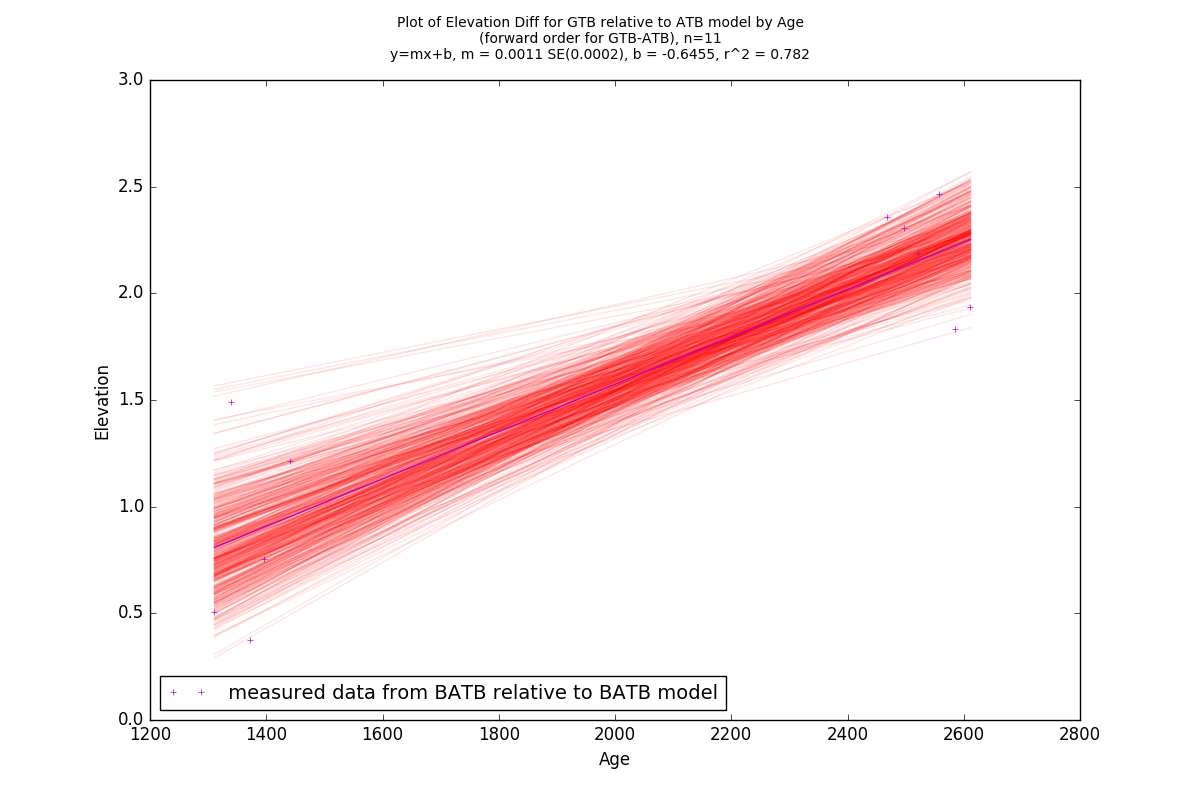
\includegraphics[width=0.9\linewidth]{data/gias/theGIA_GTB_relative_to_ATB.png}
	\caption{Differences in elevation measured from the GTB data to the ATB model}
	\label{fig:gias_GTBxATB}
\end{figure}
\newpage


\begin{figure}[h]
	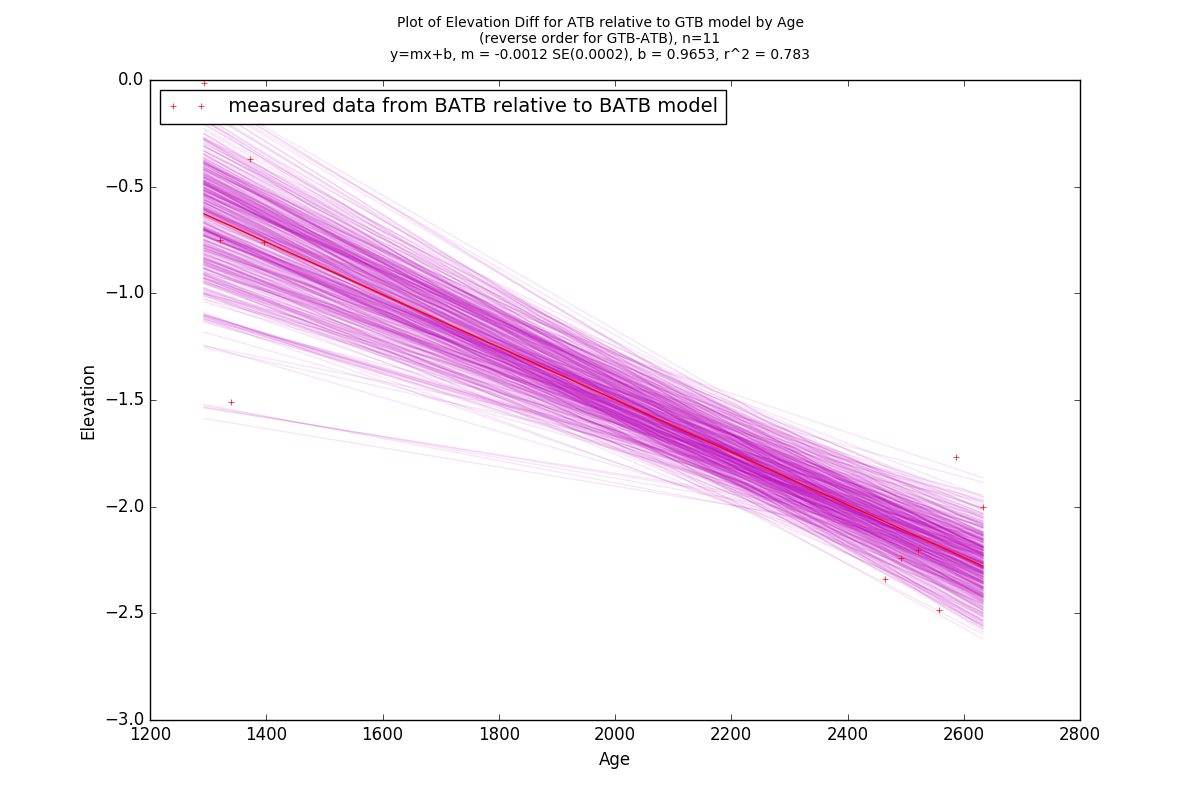
\includegraphics[width=0.9\linewidth]{data/gias/theGIA_ATB_relative_to_GTB.png}
	\caption{Differences in elevation measured from the ATB data to the GTB model}
	\label{fig:gias_ATBxGTB}
\end{figure}
\newpage










\begin{figure}[h]
	\makebox[\textwidth]{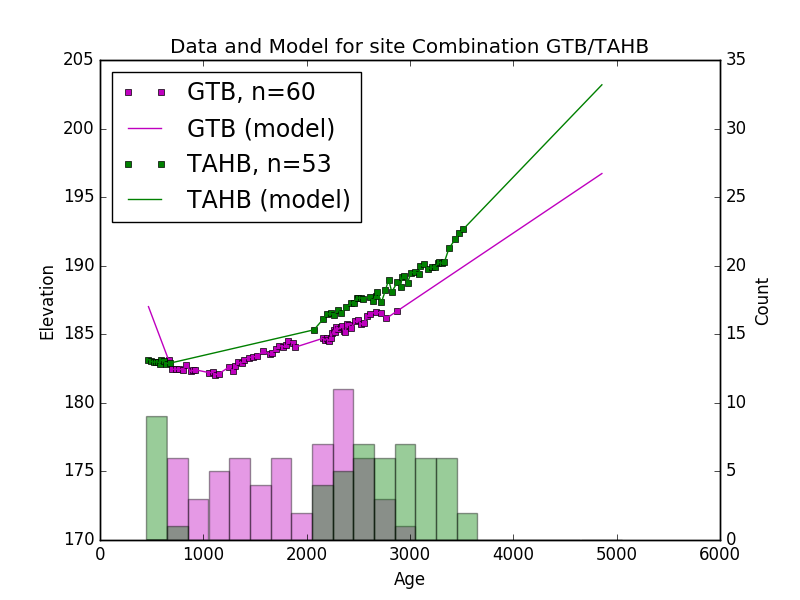
\includegraphics[width=0.72\paperwidth]{data/GTB-TAHB_DataAndModel.png}}
	\caption{GTB-TAHB raw data with linear interpolation model}
	\label{fig:data_GTBxTAHB}
\end{figure}
\newpage

\begin{figure}[h]
	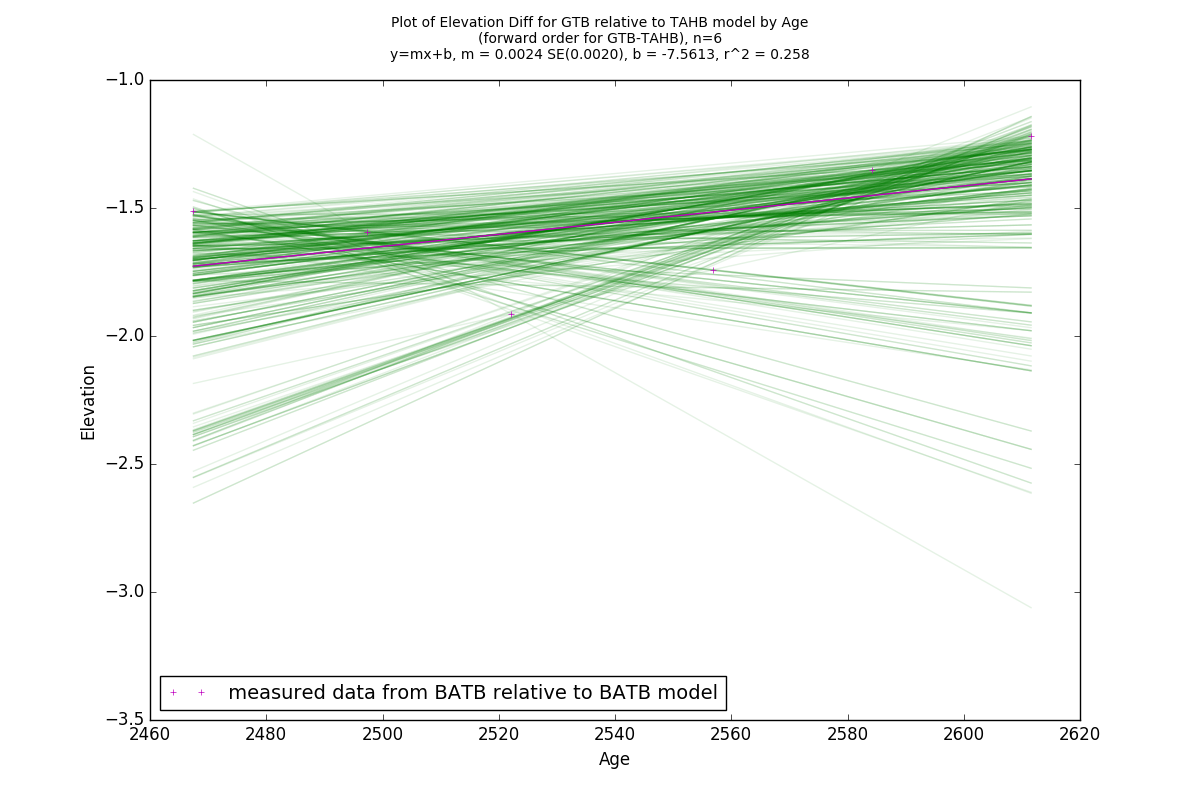
\includegraphics[width=0.9\linewidth]{data/gias/theGIA_GTB_relative_to_TAHB.png}
	\caption{Differences in elevation measured from the GTB data to the TAHB model}
	\label{fig:gias_GTBxTAHB}
\end{figure}
\newpage


\begin{figure}[h]
	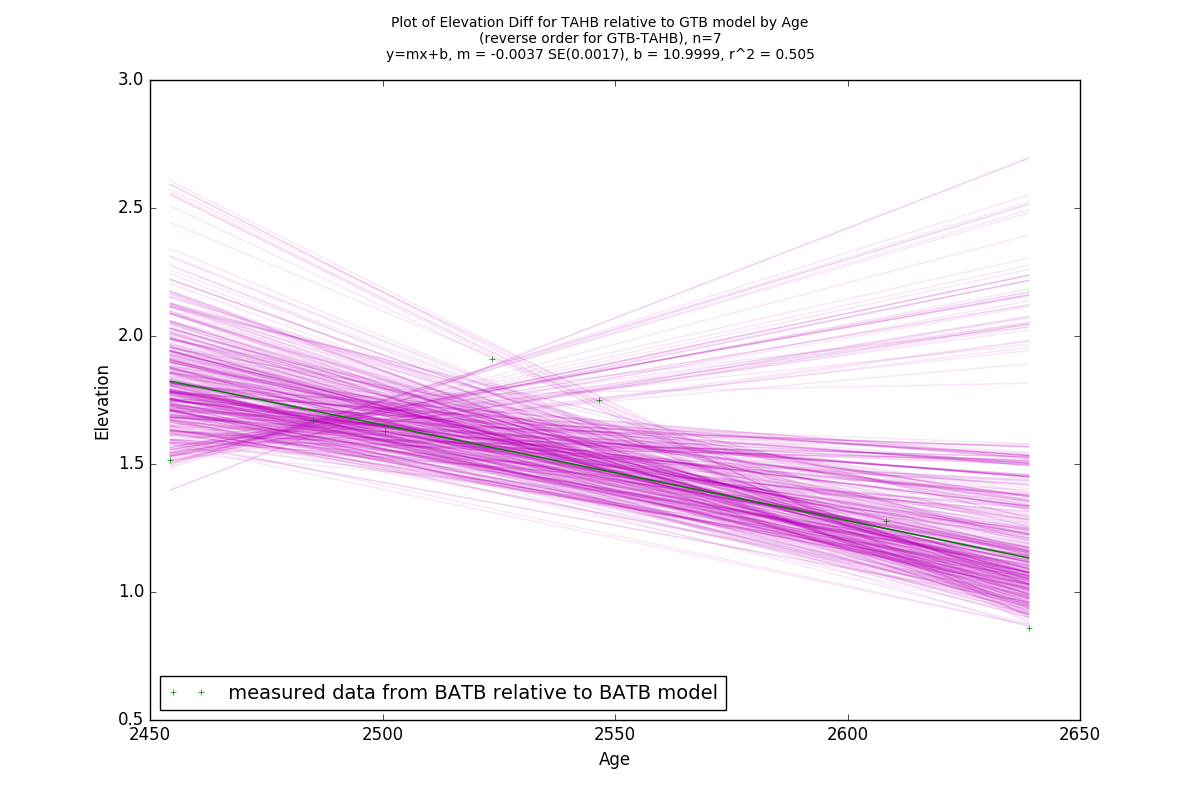
\includegraphics[width=0.9\linewidth]{data/gias/theGIA_TAHB_relative_to_GTB.png}
	\caption{Differences in elevation measured from the TAHB data to the GTB model}
	\label{fig:gias_TAHBxGTB}
\end{figure}
\newpage


\begin{figure}[h]
	\makebox[\textwidth]{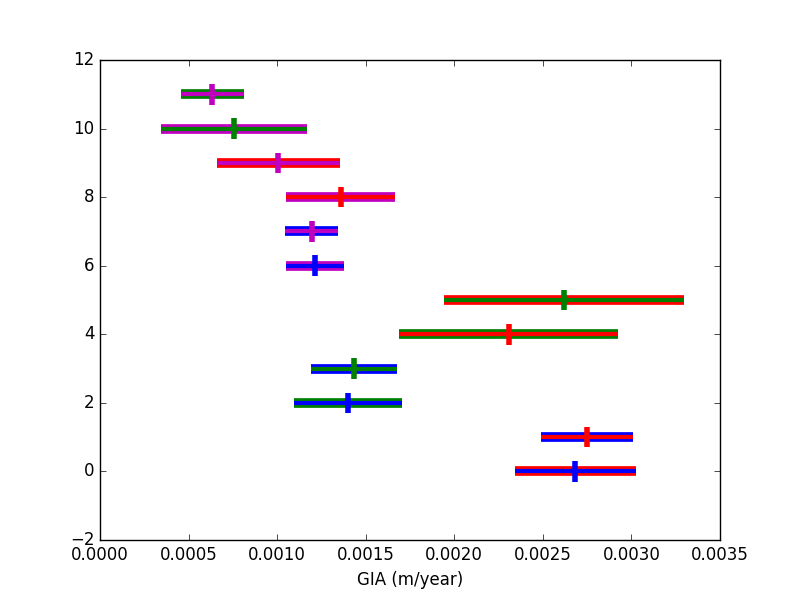
\includegraphics[width=0.6\paperwidth]{data/intervals.png}}
	\caption{95p Confidence intervals on GIA rates obtained from site comparisons}
	\label{fig:intervalsGIA}
\end{figure}


\newpage








\end{document}
